\documentclass[12pt]{article}
\usepackage{geometry}
\usepackage{amsmath}
\usepackage{mathtools}
\usepackage{amssymb}
\usepackage{enumitem}
\usepackage{fancyhdr}
\usepackage{tikz}
\usepackage{color}
\usepackage{xspace}
\usepackage{thumbpdf}
\usepackage{listings}
\usepackage{verbatim}
\usepackage{hyperref}
\usepackage{booktabs}
\usepackage{colortbl}
\usetikzlibrary{trees}
\usetikzlibrary{shapes,arrows}
\pagestyle{fancy}

\newcommand{\xref}[1]{\S\ref{#1}}
\definecolor{darkred}{rgb}{0.7,0,0}
\definecolor{darkgreen}{rgb}{0,0.5,0}
\hypersetup{colorlinks=true,
	linkcolor=darkred,
	citecolor=darkgreen}

\lstset{
	basicstyle=\ttfamily,
	mathescape
}

\lstdefinestyle{customc}{
	belowcaptionskip=1\baselineskip,
	breaklines=true,
	% xleftmargin=20pt,
	language=matlab,
	% frame=L,
	escapeinside={@}{@},
	showstringspaces=false,
	basicstyle=\small\ttfamily,
	keywordstyle=\bfseries\color{green!40!black},
	commentstyle=\itshape\color{purple!40!black},
	%identifierstyle=\color{blue},
	stringstyle=\color{orange},
	% directivestyle=\color{brown},
	%numbers=left,
	%numberstyle=\tiny\color{gray}
}

\lstdefinestyle{customctable}{
	aboveskip=-\medskipamount,
	belowskip=-\medskipamount,
	language=C,
	escapeinside={@}{@},
	showstringspaces=false,
	basicstyle=\scriptsize\ttfamily,
	keywordstyle=\bfseries\color{green!40!black},
	commentstyle=\itshape\color{purple!40!black},
	%identifierstyle=\color{blue},
	stringstyle=\color{orange},
	directivestyle=\color{brown},
}

\makeatletter
\renewcommand*\env@matrix[1][*\c@MaxMatrixCols c]{%
	\hskip -\arraycolsep
	\let\@ifnextchar\new@ifnextchar
	\array{#1}}
\makeatother

\newcommand*{\vertbar}{\rule[-1ex]{0.5pt}{2.5ex}}
\newcommand*{\horzbar}{\rule[.5ex]{2.5ex}{0.5pt}}

\textheight=8.5in

\newcommand{\hongzi}[1]{{{\color{red}(HM: #1)}}}

\lhead{6.854 Pset 9}
\chead{Hongzi Mao \:\: \footnotesize{co. w/} Linus Hamilton, Kevin Yang, Calvin Lee}
\rhead{Nov 9, 2016}

\begin{document}
\section*{Problem 1}
\paragraph{(a)} The algorithm can be achieved in linear time. Suppose all nodes and are initially randomly stored, we build a list while traverse through all nodes once. During the traversal, for each node, we build another list storing all the edges connecting it, the node at the other, and an extra field associated with the nodes indicating whether the node is occupied or not. The preprocessing step takes $O(m + n)$ time. In the matching, we traverse the nodes in the list, and greedily chose from the list of the node to connect to the other not-yet-connected node, and mark both nodes occupied. The traversal step takes $O(m + n)$ time because every edge and node in the graph is at most visited once\footnote{The edge can be deleted from the list once it is occupied, so that it won't be visited again by the other node. Even if not deleted, every edge is visited twice, still linear time.}. Therefore the algorithm completes in linear time.

Greedy algorithm is 2-approximation of the optimal solution. For any edge $e(u, v)$ in OPT, greedy algorithm picks at least one of the endpoint to connect to possibly some other edge, namely $e(u, v')$ or $e(u', v)$ or both, because otherwise the algorithm would have greedily picked these two endpoints and connect to this edge, as they are both not connected anywhere. Therefore, at least half of the endpoints are used, which implies 2-approximation. 

\paragraph{(b)} The algorithm can be implemented in $O(m\:log\:n)$ time. Suppose all nodes and edges are initially randomly ordered. For each node, we sort and find the largest weight edge, this takes $O(n\: log\: n)$ time. Then for every node, we pick the largest weight edge, if the other node has been selected we compare and get the larger weight edges (this step can cascade) and the total running time is $O(n\: log\: n)$ (edges only need to be sorted once). The result will be edges of matching in the decreasing order. The total running time for traversing all nodes will then be $O(m\:log\:n)$.

The 2-approximation of greedy algorithm is similar for part (a). For any edge $e(u, v)$ being selected by the greedy algorithm, at best OPT would choose some other edges for $u$ and $v$, $e(u, v')$ and $e(u', v)$. Notice that both $e(u, v')$ and $e(u', v)$ would have smaller weight than $e(u, v)$, otherwise the greedy algorithm would have chosen the other edge. Therefore, OPT is at best twice better than greedy, and the 2-approximation follows.

\paragraph{(c)} In the general case, we still pick the largest weight edge of each node and the above arguments similarly holds. The running time for the algorithm is still $O(m\:log\:n)$. 

This greedy algorithm is still a 2-approximation algorithm. Consider each time the edge $e(u,v)$ being selected by the greedy algorithm will be removed from the graph. In OPT, at best it instead removes $e(u', v)$ and $e(u, v')$ (i.e., OPT picks these edges in the matching). Notice that both $e(u', v)$ and $e(u, v')$ have smaller weights than $e(u,v)$, otherwise the greedy algorithm would have chosen the other edges. Now at each step, greedy algorithm at most screws up half of the weights, and therefore it implies 2-approximation in the general case.

\pagebreak
\section*{Problem 2}
\paragraph{(a)} The idea is that when the traveling time only involves small integers, we can use an algorithm mixed dynamic programming with Dijkstra to find the path with smallest traveling time within the gasoline consumption. 

\begin{figure}[h!]
	\centering
	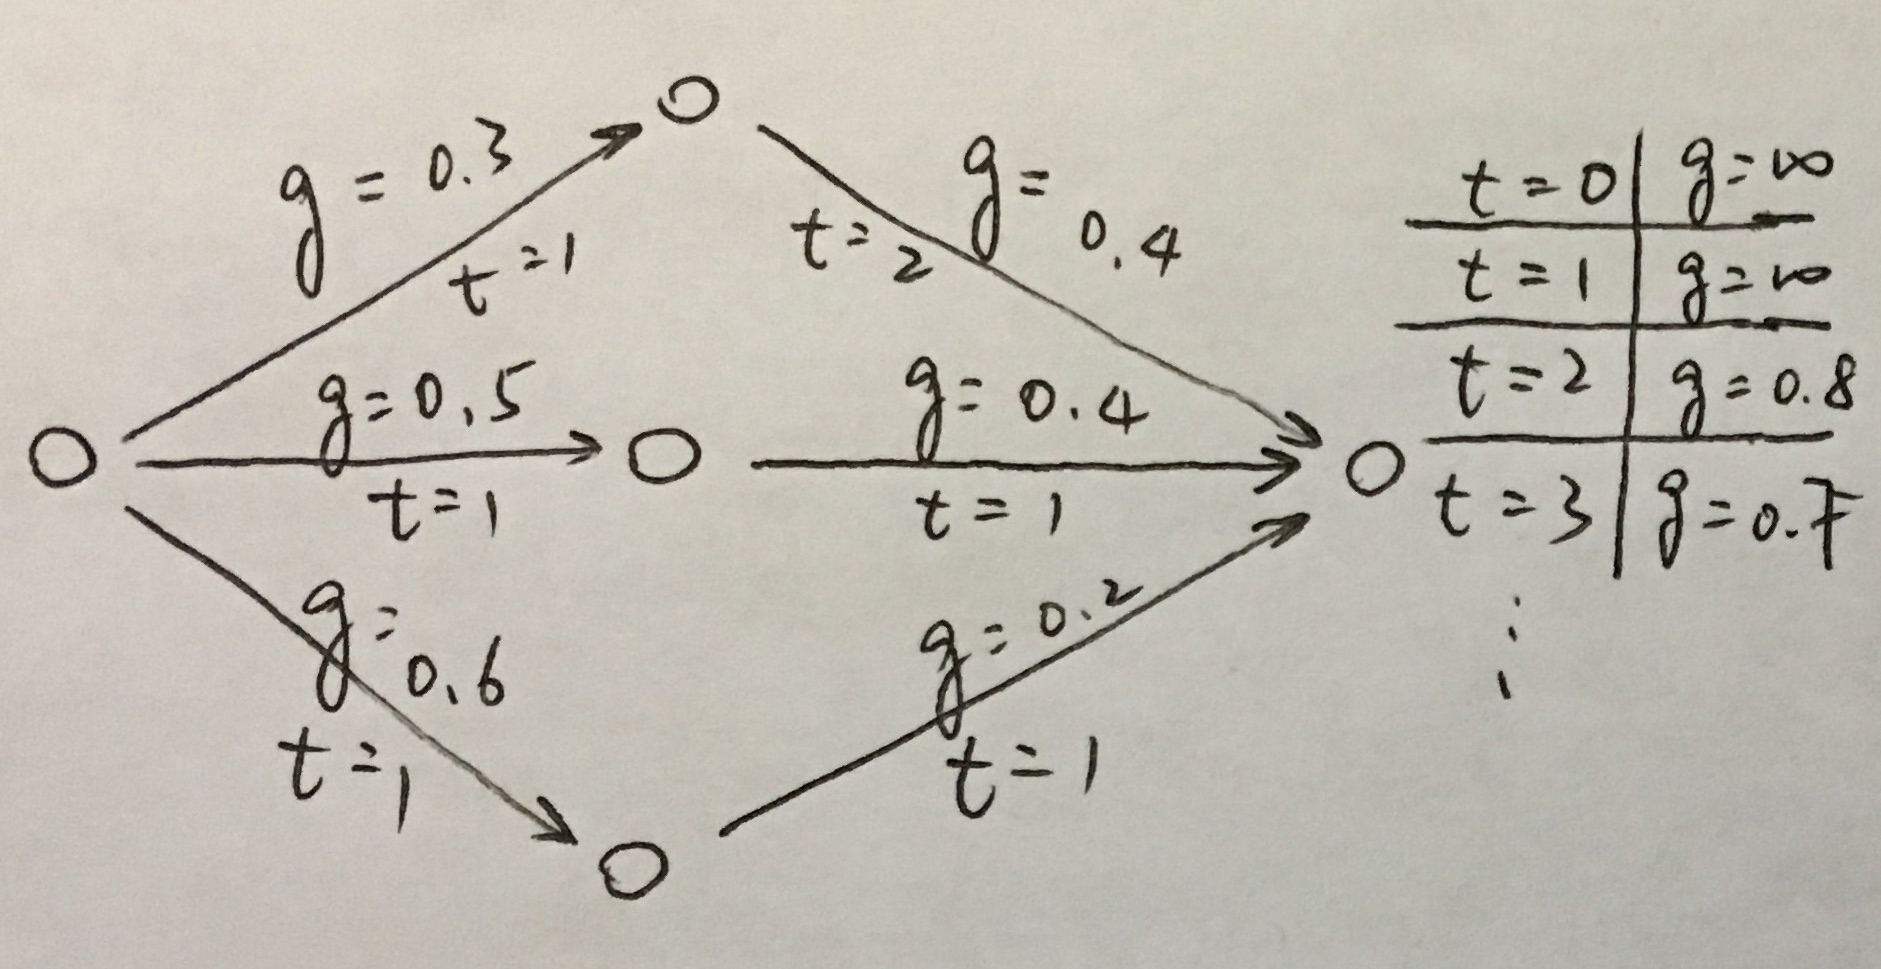
\includegraphics[width=0.6\textwidth]{2-1.jpg}
	\caption{\small{On each edge, $g$ denotes the gasoline consumption and $t$ denotes the traveling time. The table on the node saves the information of reaching to this node of traveling time $t$, how much gas is required.}}
	\label{fig:2-1}
\end{figure}

For each node, we associate a table with it, storing the information of using the time to travel to this node, how much gasoline it is at least needed. If the time is not feasible, or the gasoline consumption is over the limit, the table would store infinite gasoline in that entry. We use a Dijkstra algorithm mixed with dynamic programming to fit in the entries in the table. The idea is that once an entry in a node table is filled in, it will not be modified. Specifically, since the graph is acyclic, like in Dijkstra, we maintain a global searched traveling time $\tau$\footnote{If needed, we can also mark each entry in the node, whether or not we have searched the outgoing edge, to avoid duplication because each edge can be revisited for retrieving different entry in the table.}. Initially all tables in the nodes are initialized with $g=\infty$. Then every time we fill in the entry of the table(s) on a node (or nodes), if the traveling time to this node is the globally smallest but larger than $\tau$ and the gasoline consumption is not over the limit. This is computed from previous nodes based on the available traveling time on their tables, where we add the traveling time and gasoline consumption on current edge and we break ties by favoring smaller gasoline consumption. Then we increase the current searched $\tau$ to the time we just searched. The algorithm terminates when an entry in the destination node is filled with gasoline consumption within the limit. 

This way, we will fill in the tables in all the nodes, with information of if we were to take time $t$ to this node, how much gasoline $g$ would it take. Dijkstra makes sure the search is `shortest path' based, meaning that once an entry is filled in, it would not be modified. The dynamic programming search makes sure the table is filled in based on the time and gasoline from last node's table. 

Since we assume the traveling time is a small integer, the size of the table is manageable. Given $m$ edges, and largest traveling time $q$, the size of the table is bounded by $mq$. Since each time we will fill in at least one entry of a table using the algorithm above, which would not modify a filled table entry. Given there is $n$ nodes, the running time of the algorithm is $O(nmq)$.

\paragraph{(b)} For an approximation we can have a integer bound (the small integer we have in (a)), and then round all traveling time in the integers in the bound. In particular, for traveling time outside the bound, we will round it to the maximum boundary. Then we can use (a) to solve this problem. Since the gasoline consumption is kept the same in the rounding (still fractional), when taking the path returned from (a) algorithm, and using the original traveling time, the solution is still feasible. 

The approximation of this rounding is bounded by first the rounding down of the traveling time larger than the integer bound, and second the granularity (we can first scale the numbers than round to integers) when we round numbers to integers. 

For rounding down, since we take the same path and use the original traveling time, the source of the error come from the edges above the integer bound. More specifically, this will happen when there exists path of traveling time in the original smaller than the one returned in the rounding. This means after the rounding, the path with traveling time smaller in the original graph, becomes larger than the rounded path. Suppose the integer bound is $p$ and the max traveling time in the original graph is $P$. The largest gap would be $m(P-p)$ (the real optimal is $\sim mp$ and the algorithm returns $mP$) To bound this error, we need to make $p$ very close to $P$, in fact, within $\epsilon/m$ close to $P$. This is the first factor in FPAS.

For the second case, we first scale up the traveling time (therefore the $P$ in first part needs to enlarge as well) then we round the number to the integer. The source of error in this case is from the granularity. On each edge, the traveling time is at most off by $1/r$ where $r$ is the scaling factor. In the worst case, the optimal path has its traveling time rounding up on each edge and some other path has traveling time rounding down on each edge. Therefore, in total the error can be at most $m/r$. To bound the error in this case, we need to choose the scaling factor $r = O(m/\epsilon)$.

In total, to achieve error within $\epsilon$, we need to scale the traveling time by $O(m/\epsilon)$ and set the integer bound to an integer within $\epsilon/m$ to the max traveling time on the edges. Then we use (a) to return the feasible path and return the traveling time in the original graph as an approximation.

\paragraph{(c)} Since the traveling time and gasoline consumption are all positive, there is no point traveling in a cycle. In the plain solution of (a), traveling in a cycle will increase the traveling time and gasoline consumption, therefore this won't modify an existing entry in the table as traveling time increases, also this will terminate because we only have finite entries in the table (traveling in a circle will eventually hit the limit of $mq$), and the Dijkstra algorithm ensures this traveling in a loop won't affect other entries (shortest path is populated out before traveling back to the node).

In fact, we can also prevent cycling from happening in the beginning. Before we fill in an entry in the table, if we find out that the entry we are about to fill in, has \emph{both} the traveling time and the gasoline consumption larger than some existing entry, there is no need to add in the entry. This is because the only reason we may need to add in a larger traveling time, is that it may have smaller gasoline consumption. This will prevent the loop from being recorded as the traveling time and gasoline consumption is larger than what we had when we first visit the node\footnote{Besides cycles, this also saves us from doing unwanted work, for the same reason that may may need to add in a larger traveling time only because it may have smaller gasoline consumption.}.

\newpage
\section*{Problem 3}
\paragraph{(a)} The maximum total running time of all jobs are bounded by $T = \sum_j p_j$. Suppose job $j$ completes at time step $t$, then indicator $x_{jt} = 1$ and $0$ for other values. The ILP can be written as\footnote{Notice that the precedence constraints could have been written as $\sum_{t=0}^T (t+p_j) x_{it} \leq \sum_{t=0}^T t x_{jt}$, since each job $j$ should finish at least its running time $p_j$ after the completion time of its predecessor. But this constraint is absorbed in the third constraint, that at most one job can run at a time. Also, it can be equivalently written as $\sum_{t=0}^\tau x_{it} \leq \sum_{t=0}^\tau x_{jt}, \: \forall i \in A(j), \forall \tau$, which is better to analyze in LP relaxation case.}
\begin{align*}
\text{minimize}\:\:& \sum_j{w_j}\sum_{t=0}^{T} t x_{jt}\\
\text{subject to}\:\:& \sum_{t=0}^T x_{jt} = 1,\: \forall j \:\:\:\:\:\:\:\:\:\:\:\:\:\:\:\:\:\:\:\:\:\:\:\:\:\:\:\:\:\: \text{(every job needs to complete)}\\
&\sum_{t=0}^T t x_{it} \leq \sum_{t=0}^T t x_{jt}, \: \forall i \in A(j) \:\:\: \text{(precedence constraints)}\\
& \sum_{t=0}^{\tau} \sum_{j} x_{jt}p_{j} \leq \tau, \: \forall \tau \:\:\:\:\:\:\:\:\:\:\:\:\:\:\:\:\:\: \text{(only one job can run at a time)}\\
& x_{j,t} = \{0, 1\}
\end{align*}

\paragraph{(b)} Notice that we have from part (a) $\sum_{t=0}^T x_{jt} = 1$, and now $x_{jt}$ can be fractional. The half completion time can be defined\footnote{Can be thought of as a way to find $h_j$, I found it a bit vague in the problem.} as the \emph{smallest} time step at which $\sum_{t < h_j} x_{jt} \geq \sum_{t \geq h_j} x_{jt}$. In the half completion time, since half of the work is completed, we also enforce $\sum_{t\geq h_j} x_{jt} \geq 1/2$, and we will have $\sum_{t < h_j} x_{jt} = \sum_{t \geq h_j} x_{jt} = 1/2$. Then we have 

\begin{align*}
\bar{C_j} = \sum_t t x_{jt} &= \sum_{t< h_j} t x_{jt} + \sum_{t\geq h_j} t x_{jt}\\
& \geq \sum_{t< h_j} t x_{jt} + \sum_{t\geq h_j} h_j x_{jt}\\
&\geq \sum_{t\geq h_j} h_j x_{jt}\\
&= h_j\sum_{t\geq h_j} x_{jt}\\
&= h_j/2
\end{align*}

\paragraph{(c)} The LP relaxation enforces the precedence of half-way run time. This can be shown by contradiction. Suppose for a job $i \in A(j)$ of job $j$, and we assume job $j$ runs before its predecessor $i$, i.e., $h_i > h_j$. Notice that the second constraint in (a) can be equivalently written as 
\begin{align*}
&\sum_{t=0}^\tau x_{it} \leq \sum_{t=0}^\tau x_{jt}, \: \forall i \in A(j) , \forall \tau
\end{align*}
We can equivalently run the LP relaxation on this constraint. Then we will have $\sum_{t=0}^{h_j} x_{it} \leq \sum_{t=0}^{h_j} x_{jt} = 1/2$. Now notice that in (b) we know $h_i$ is the \emph{smallest} time point, that makes $\sum_{t=0}^{h_i} x_{it} \geq 1/2$, this contradicts with the assumption that $h_i > h_j$. Therefore no job can run before its precedents.

\paragraph{(d)} We sort the job index $\{1, 2, 3, ...\}$ by their half completion time, hence $h_1 \leq h_2 \leq h_3 \leq \dots$ For a specific job $j$, from the second last constraint in (a), we can replace $\tau$ with $h_j$, then we have 
\begin{align*}
& \sum_{t=0}^{h_j} \sum_{j} x_{jt}p_{j} \leq h_j\\
\implies & \sum_{t=0}^{h_j} \sum_{i=1}^{j} x_{it}p_{i} \leq h_j\\
\implies & \sum_{i=1}^{j} p_{i} /2 \leq h_j\\
\implies & \sum_{i=1}^{j} p_{i} \leq 2h_j\\
\implies & \sum_{i=1}^{j} p_{i} \leq 4 \bar{C_j}
\end{align*}
From (c) we know, any precedent $i$ of $j$ should have their half completion time $h_i$ earlier than $j$. Therefore $\sum_{i=1}^{j} p_{i}$ upper bounds the completion time of $j$. From the derivation above, we know $j$'s actual completion time is at most $4 \bar{C_j}$.

\paragraph{(e)} First we write the constraint is listed in part (a). Then we replace the last constraint for LP relaxation to $x_{j,t} \in [0, 1]$. Next, we solve the LP problem and calculate the half-way runtime as in (b). We schedule the job in the half time as in part (c) and the feasibility is preserved. The scheduling result is at most $4$ times worse than optimal as in (d). Therefore we arrive at $4$-approximation, which is a constant factor approximation scheme for this scheduling problem.

\newpage
\section*{Problem 4}
\paragraph{(a)} If the number of types of all items is bounded by a constant $k$, a kind of like brute force algorithm can solve it in polynomial time. First, notice that the total number of different combinations of items is polynomially bounded. A very loose bound\footnote{More careful tricks in combinatorics may give a better bound but we only care \emph{polynomial} time here.} can be computed as follows. For a subset of size $m \leq n$, all items of size type, it has $k$ possibilities; $m-1$ items of 1 kind, $1$ item of a different kind, this has $k^2/2$ possibilities. Continuous these, the possibility is bounded by $k!$ and since we assume $k$ to be constant this value is bounded. On the other hand, for the number of subset with different number on each kind, it is bounded by $O(n^k)$, because this is bounded by counting the possibility of putting $k$ separation among $n$ items (allows separations have no items in between, which is $(n+k)$ chooses $k$). Therefore, the total possibility of subsets are polynomially bounded. 

Then, suppose we tried our best for putting items into $i$ bins. Then there is a polynomial time algorithm for $i+1$ bins. Specifically, every time we look into the items left after putting things into $i$ bins and try out all subsets (bounded by a polynomial number) and put the best we can do to the $i+1$ bin. Since starting from $0$ bins, we have every item to find a subset and pack, we can boot-strap. At each step, the time is bounded by the total number of possible subsets, bounded by a polynomial number, and the total number of steps is bounded by $n$, the algorithm can return in a polynomial time.

\paragraph{(b)} For each new item with size smaller than $\epsilon$, we check if we can put in the current bin, and put it in a new bin if not possible. For the current bin (and newly added bin), if we can not put a new item into it, we stop checking it in lateral runs. Therefore, the running time is linear with total number of current bins and total number of items to add. 

Since we check current $B$ bins before the new bins, the only case that a new bin is needed is that an item can not be put in the bin. Notice that all remaining items have size less than $\epsilon$, this implies the current bins that are ceased checking have items with total size at least $1 - \epsilon$. Also, the sum of all items is bounded by $B^*$ (all items seamlessly put in $B*$ bins), total number of bins needed in this algorithm is $\lceil \frac{B^*}{1-\epsilon}\rceil$.

Now consider two cases. If $\epsilon < 1/2$, we will have 
\begin{align*}
\lceil \frac{B^*}{1-\epsilon}\rceil \leq 1 + \frac{B^*}{1-\epsilon} \leq 1 + (1 + 2\epsilon) B^*,
\end{align*}
as desired in max$(B, 1 + (1 + 2\epsilon) B^*)$ result.

If $1 \geq \epsilon \geq 1/2$, in this case each of the $B$ bins already contain items of total size larger than $\epsilon \geq 1/2$, namely at least half full. Now, consider in the algorithm that an item can not be inserted in a bin and is therefore inserted into a new bin. For these two bins, the total capacities is $2$, and the size of items in them is larger than $1$, otherwise the item would have been inserted into the first bin, no need for a new bin. Therefore, we know all bins at the end is at least ``half-full'' on average. Therefore 

\begin{align*}
B \leq 2B^* \leq (1 + 2\epsilon)B^* < 1 + (1 + 2\epsilon)B^*.
\end{align*}
which also meet the desired result max$(B, 1 + (1 + 2\epsilon) B^*)$.

\paragraph{(c)}
It is a different case with job scheduling, over here the scaling of those item size would change the number of bins required. In fact a small change can lead to a significant difference in the resulting number of bins. It is about fitting in the bin or not, consider a bin very close to full and messing up the items there can have cascade effect and double the number of bins. In job scheduling the constraints are softer than this and the objective is different (minimizing the load, instead of number of machines being used).

\paragraph{(d)} We set aside the items in $S_1$, and put each of them in a new dedicated bin. Then we will show the remaining items can still fit into the original bins. Since the newly added bins are for the $n/k$ items in $S_1$, it only increases the optimal number of bins by $n/k$. 

For the remaining items, it is enough to `promote' to bins used previously by higher group and enough to fit all of them. This is because each item changes its size at most to the size of the $n/k$ item in front of it before the grouping (except the first group, which we already set aside). More specifically, $\forall i \notin S_1$, item$_{i, after\:grouping}$ $\leq$ item$_{i - k/n, before\:grouping}$. This means, we can put all items after grouping to the bins following the index shift of $n/k$ and do not violate capacity constraint, since the sizes are smaller than the items originally there. 

As stated above, therefore the total number of bins increase by $n/k$. 
\paragraph{(e)} Let $m$ be the number\footnote{It can be the case that every item has size less than $\epsilon$, then we can reduce $\epsilon$ to make $m$ non-zero, this would achieve a smaller error in the result.} of items has size greater than $\epsilon$, for part (d), we set $k = \frac{n}{m\epsilon^2}$. Then from (d) we will have the total number of bin is bounded by 

\begin{align*}
B \leq \lceil B^* + \frac{n}{k} \rceil = \lceil B^* + n/\frac{n}{m\epsilon^2} \rceil= \lceil B^* + m\epsilon^2 \rceil
\end{align*}

Notice that for all $m$ items, summing over $\epsilon$ can be bounded by $B^*$ as 
\begin{align*}
m\epsilon \leq B^*
\end{align*}

Therefore we have 
\begin{align*}
B \leq \lceil B^* + \frac{n}{k} \rceil = \lceil B^* +  m\epsilon^2\rceil \leq \lceil B^* + \epsilon B^*\rceil \leq (1+\epsilon)B^* + 1
\end{align*}

This follows the result in (b) that $B \leq \text{max}(B, 1 + (1+\epsilon)B^*)$. From part (b) we also know we can add the items (the feasibility is shown in (d)) in these bins in linear time to the number of items and number of bins. Hence the overall algorithm returns an approximation within $1 + (1+\epsilon)B^*$ in polynomial time.
\newpage
\section*{Problem 5}
\paragraph{(a)} If we know where the bridge is and suppose the distance to the bridge is $d$, we can go to the bridge directly and cost $d$. Now we use the following `search' algorithm to iteratively find the bridge. 

Start from origin $0$, we first go to $1$, then from $1$ to $-2$, then to $4$, then to $-8, 16, -32, 64, \dots$ In other words, traversing the origin, each time we walk $-2^{i} + 2^{i-1}$ to do the search. Since the bridge is in a finite integer point, this search algorithm will always terminate. 

For the bridge at point $d$, this algorithm needs jump back and forth to find it. Specifically, it takes ${\lceil log\:d\rceil}$ iterations to find the right interval. And in this run, it takes $d$ to go to the right place of the bridge. In the worst case, this iteration starts in the wrong direction and we walk to the wrong half back to the origin first, this takes extra searching $2^{\lceil log\:d\rceil}$. In total, this takes 

\begin{align*}
\sum_{i=0}^{\lceil log\:d\rceil} \left[2^{i-1} + 2^{i}\right] + d + 2^{\lceil log\:d\rceil} &\leq \sum_{i=0}^{log\:d + 1} \left[2^{i-1} + 2^{i}\right] + d + 2^{log\:d + 1}\\
&\leq 2^{log\:d + 1} + 2^{log\:d + 2} + d + 2^{log\:d + 1}\\
&= 2\times 2^{log\:d} + 4\times 2^{log\:d} + d + 2 \times 2^{log\:d }\\
&\stackrel{O(\cdot)}{\simeq} 2d + 4d + d + 2d\\
&= 9d
\end{align*}

Compared with the offline optimal algorithm with cost $d$, this searching algorithm takes $9d$. Hence this algorithm is $9$-competitive.

\paragraph{(b)} Notice that in the worst case above we need to walk extra $2^{\lceil log\:d\rceil}$ steps to find the bridge, because in that iteration we start in the wrong direction. Now instead of initially going to the positive deterministically, we can randomly choose our starting direction. Then it means it is equally likely for us to need to walk the extra distance $2^{\lceil log\:d\rceil}$. If we end up with walking the extra, then the cost is the same as above $9d$. 

In the other half of the time, we are lucky and we found the bridge \emph{within} the iteration. This means that we don't need to walk the extra distance and walk to the other half to find the bridge. Specifically, this time it would take ${\lfloor log\:d\rfloor}$ to home in on the right region. For example, the bridge is at $3$, when we go $-1 \to 2 \to -4 \to 8$ it takes $(2^0 + 2^1 )+ ( 2^1 + 2^2) +2^2 + 3$, where there is $\lceil log_2 3\rceil$ search regions to add; but when we go $1 \to -2 \to 4$, it takes $(2^0 + 2^1) + 3$, it only has ${\lfloor log_2 3\rfloor}$ regions to add. More formally, in the better half case, we have the searching cost
\begin{align*}
\sum_{i=0}^{\lfloor log\:d\rfloor} \left[2^{i-1} + 2^{i}\right] + d &\leq \sum_{i=0}^{log\:d } \left[2^{i-1} + 2^{i}\right] + d\\
&\leq 2^{log\:d} + 2^{log\:d + 1} + d\\
&= 2^{log\:d} + 2\times 2^{log\:d} + d\\
&\stackrel{O(\cdot)}{\simeq} d + 2d + d \\
&= 5d
\end{align*}
This gives us 5-competitive algorithm. Therefore, on average case, the randomized search is $7$-competitive. 
\paragraph{(c)} My guess is instead of walking back to the origin every time, one could go directly continuously further from the current point, at some chance this can hit the bridge, instead of walking all the way back. This might boost the competitive ratio to be less than $7$. 

Also, instead of this $1, 2, 4, 8, 16, ...$ walk, we can instead do $k, 2k, 4k, 8k, 16k, ...$, where $k\in[0, 1]$ is picked randomly. The idea is that the bad things happen when adversary tries to put the point in the far end of the interval, where we are forced to waste a `round-trip'. This way on average we will be in a better competitive ratio than $7$.
\end{document}